\section{Why is Lattice Crypto important, interesting,\ldots}
\begin{frame}{Why is Lattice Based Crypto important?}{Or interesting? Or\ldots?}
    \begin{itemize}
        \visible<1->{\item It is a Post-Quantum secure Cryptosystem (PQC)}
        \visible<2->{\item It is damn fast (faster than dinosauRS cryptA)}
        \visible<3->{\item You can build anything you want from it:\\
                  Encryption, Signatures, even Hash Functions!}
        \visible<4->{\item It allows to build even one of the most hailed advanced cryptographic building block:\\
                     Fully Homomorphic Encryption (FHC) (hallelujah!)}
    \end{itemize}
\end{frame}

\section{How does Lattice Crypto work?}
\begin{frame}{Lattice Based Crypto}
    \begin{block}{Key Generation}
        \centering
        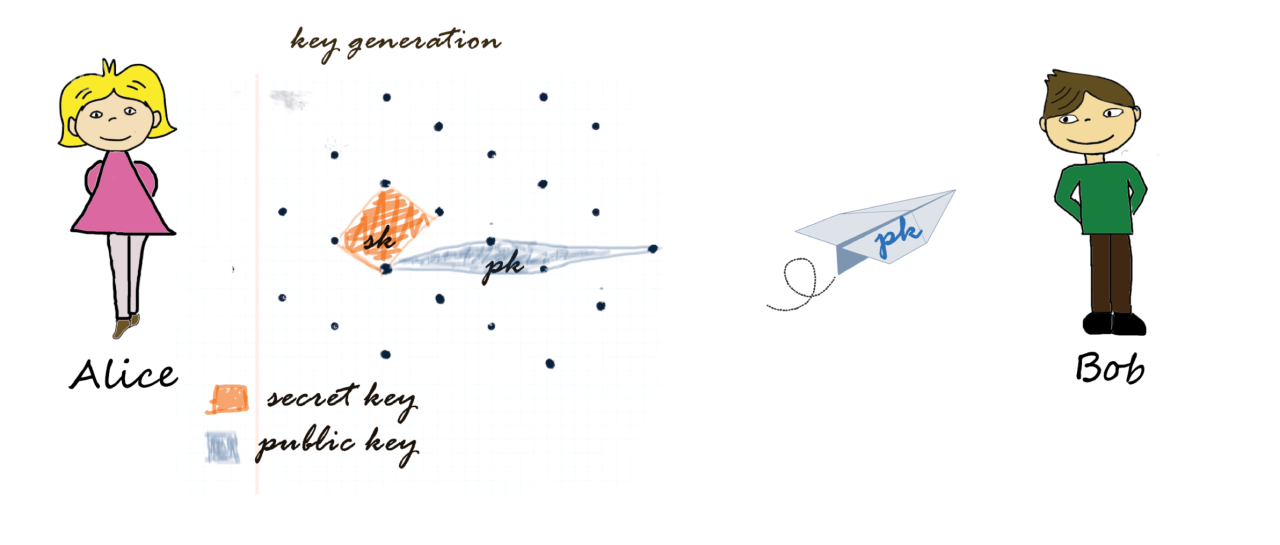
\includegraphics[keepaspectratio,width=\textwidth,height=0.8\textheight]{data/keygen}
    \end{block}
\end{frame}

\begin{frame}{Lattice Based Crypto}
    \begin{block}{Encryption}
        \centering
        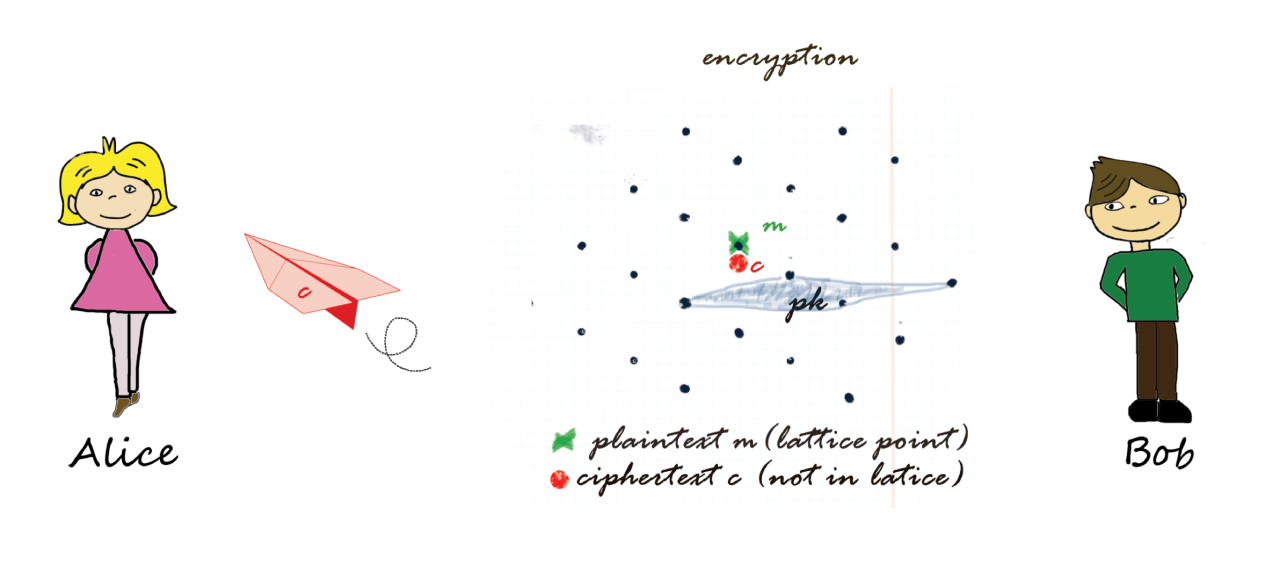
\includegraphics[keepaspectratio,width=\textwidth,height=0.8\textheight]{data/encryption}
    \end{block}
\end{frame}

\begin{frame}{Lattice Based Crypto}
    \begin{block}{Decryption}
        \centering
        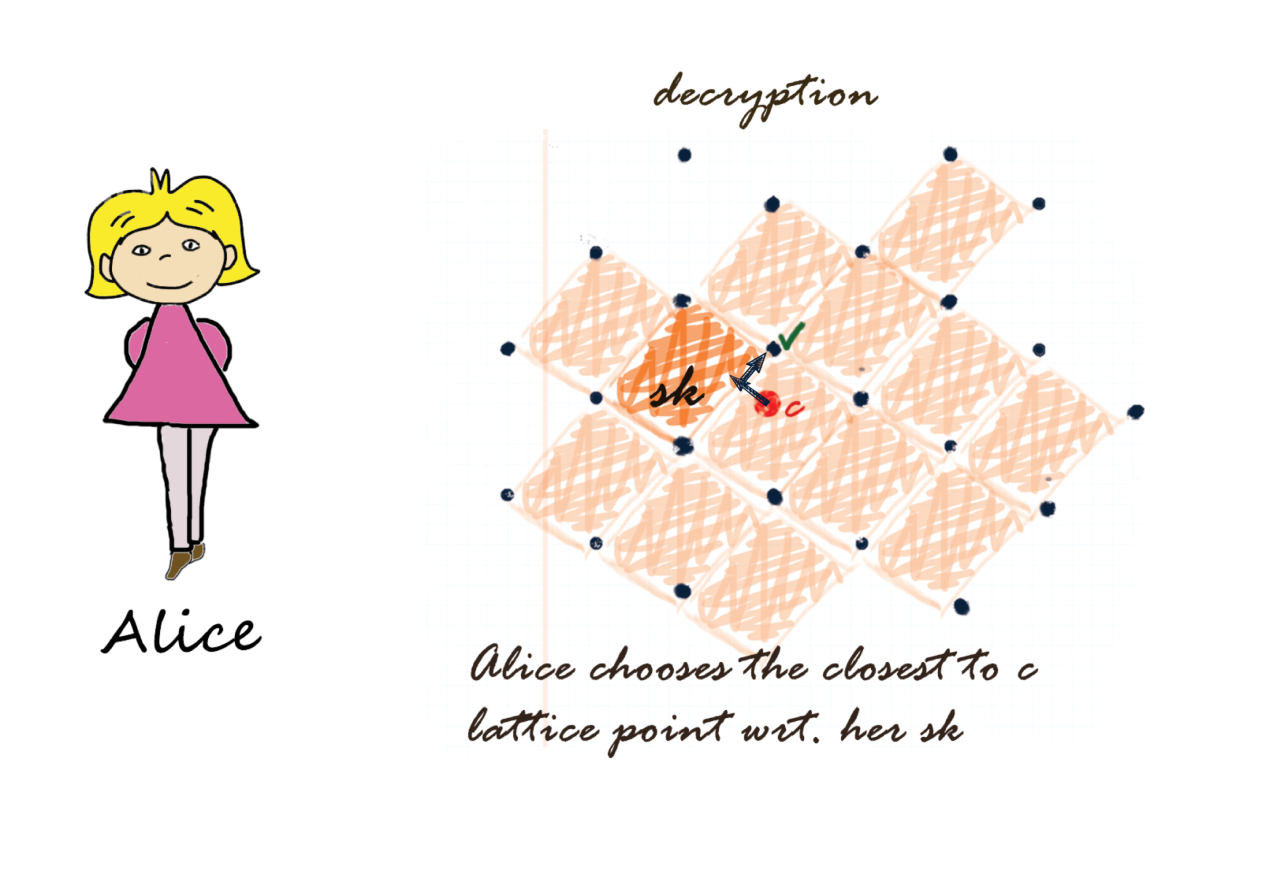
\includegraphics[keepaspectratio,width=\textwidth,height=0.8\textheight]{data/decryption}
    \end{block}
\end{frame}

\begin{frame}{Lattice Based Crypto}
    \only<1>{%
    \begin{block}{Attack}
        \centering
        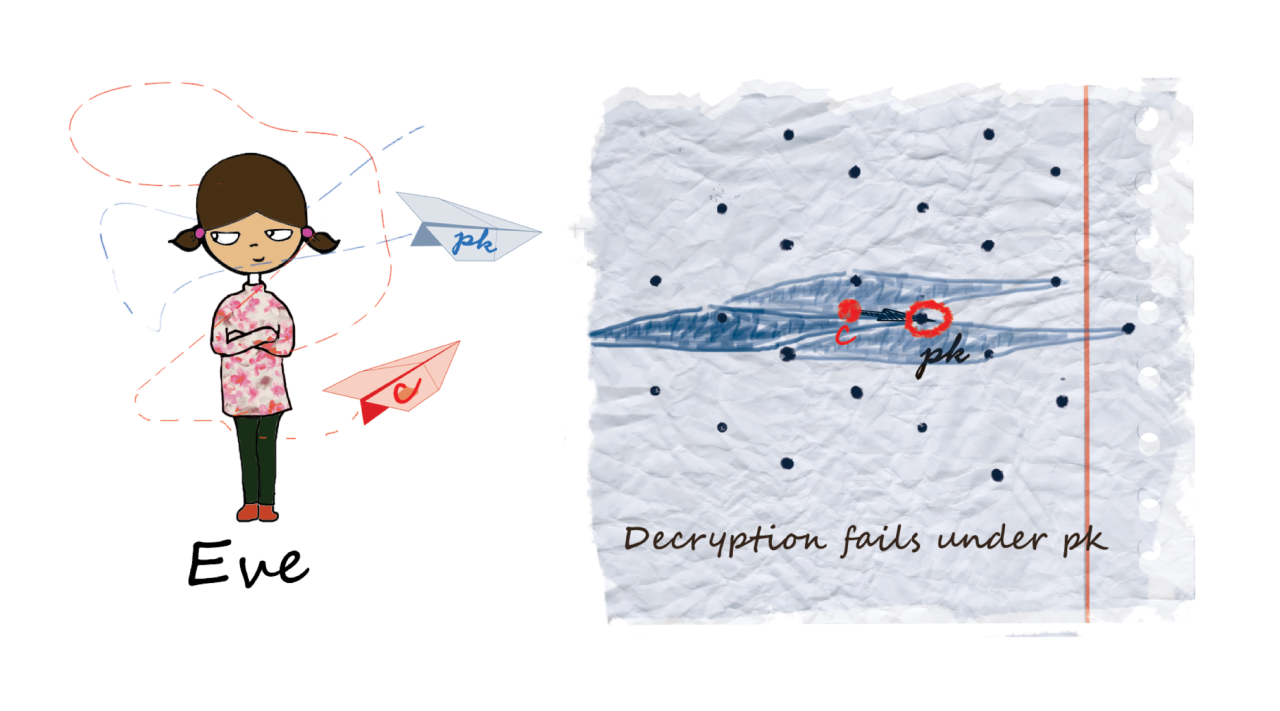
\includegraphics[keepaspectratio,width=\textwidth,height=0.8\textheight]{data/Eve}
    \end{block}
    }
    \only<2>{%
    \begin{block}{Attack}
        \centering
        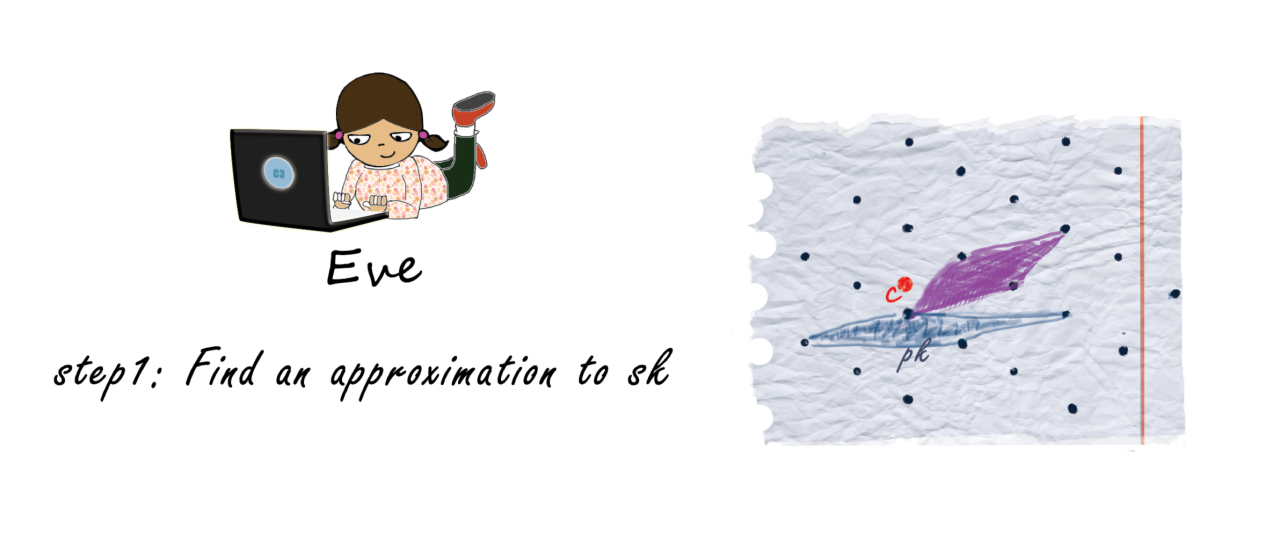
\includegraphics[keepaspectratio,width=\textwidth,height=0.8\textheight]{data/attack_step1}
    \end{block}
    }
    \only<3>{%
    \begin{block}{Attack}
        \centering
        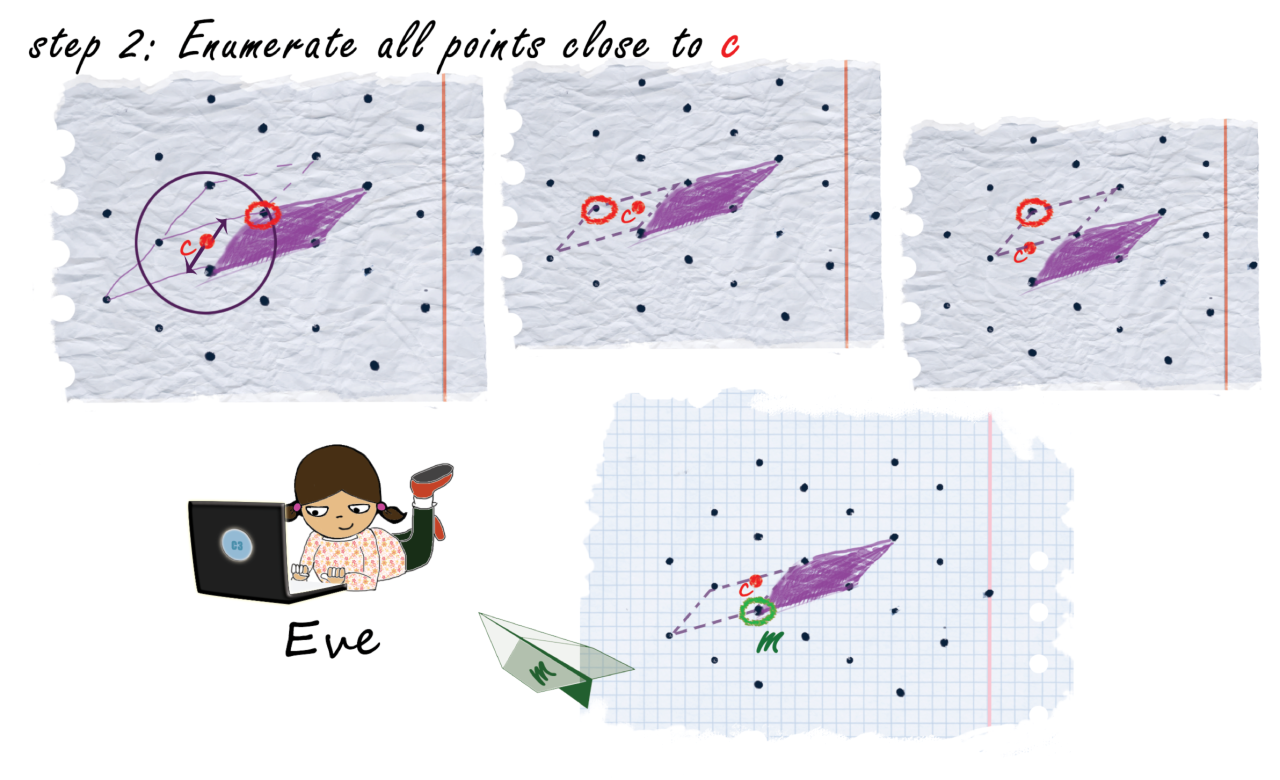
\includegraphics[keepaspectratio,width=\textwidth,height=0.8\textheight]{data/attack_step2}
    \end{block}
    }
\end{frame}
